\chapter{Introduction}

%Replace \lipsum with text.
% You may have as many sections as you please. This is just for reference.

By common opinion, a democratic society in modern world is a misnomer - an illusion often given to the "ruled" party in a nation. Two centuries after Lincoln's definition of democracy, a government-for-the-people sadly is nothing but a collection of handful of population in control of basic resources of a country (natural or artificial). Leaders in military, politics, businesses, sports and arts thus become the actual voice of a country rather than the common mass. The distribution of power in these domains are often hereditary (among close ties in family) instead of elected representatives. Interactions among the persons of these important fields are also common for their effective functioning ( or often to safeguard their self benefits.)

In this regard, accountability and transparency in government is one of the key requirements in order to obtain an ideal democratic society. Unfortunately the lack of proper knowledge about the politicians and corporates has led to new forms of "collective" dictatorship where public rights or voices are rendered ineffective.

To account for this growing problem of opacity we have tried to study the social network of Indian politicians and corporates and disemminate the information to the common public.

\textbf{Problem Statement}-
Problem of forming the social networks of Indian Politicians and Corporates, visualizing  and analysing them.

\section{Objective}
%\lipsum[1]

%You should cite papers in the following manner: Bayliss et al.~\cite{Bay1} gave an iterative method for Helmholtz equation etc.
%Similar work has been done in \cite{Bailey,Ernst,Gold3}.
We intended to complete following tasks through our project-
\begin{itemize}

    \item To \textbf{collect data from semantic web} (and other sources) to form a database ( henceforth referred to as \textbf{"knowledge base"} / \textbf{"knowledge graph"} )
    \item To create \textbf{ a neat, structured minimal error data collection } which otherwise is scattered at respective sources.
    \item To provide \textbf{ a data mashup from different fields } to further help the academecians, journalists etc.
    \item To \textbf{ monitor the top players in Indian society } - mainly in the spheres of politics and businesses in India.
    \item To \textbf{ disemminate information to public }  which brings about accountability and transparency. 
    \item  To seek answers to questions like -
        \begin{itemize}
         \item \emph{ who were the big players in Indian politics and businesses? }
         \item \emph{ Is there any influence (or possibility of it) of political field by a person in corporate field? }
         \item \emph{ How important is one politician in a network of politicians (or a businessperson in a business network)? }
         \item \emph{ Whom does actual power reside in a democracy? }
        \end{itemize}
\end{itemize}
We believe that through our work, we will be able to show how such system of inter-disciplinary data helps to spread information and find patterns and discover more knowledge.

\section{Motivation \& Related Work}

In his book \textbf{The Power Elite} \cite{Mills}, C. Wright Mills calls attention to the interwoven interests of the leaders of the military, corporate, and political elements of society and suggests that the ordinary citizen is a relatively powerless subject of manipulation by those entities. His book deals with the power elite in US. But the hierarchy he proposes is more or less the same across all countries. Power rests with the top one percent in an economy. We plan to create a watchdog for that one percent. One interesting list to accompany this direction could be the Forbes list \cite{FORBES} of 147 companies that control everything. 

French economist Thomas Piketty in his famous work \textbf{Capital in the Twenty-First Century} \cite{Piketty} focuses on wealth and income inequality in Europe and the United States since the beginning of the industrial revolution. He proposes a global system of progressive wealth taxes to help reduce inequality and avoid the vast majority of wealth coming under the control of a tiny minority. We plan to collect, integrate, visualize and open such data for Indian terrain to let data fanatics carry out sych works to understand this inequality.

British writer and historian Patrick French, in his book \textbf{India: A Potrait} \cite{French} has stated many such interesting patterns in Indian politics where he argues that almost all of the young Indian politicians in the Indian Parliament are hereditary. Infact, patterns similar to this can be seen over the entire political Indian scene. One can find interesting overlaps, family ties, social links within these power houses. In a survey, \textbf{Who owns your media?} \cite{Media}, we find that even the media is an entity of importance and most of the politicians tend to try pull their strings in this domain. Another interesting case could be Jayant Sinha's family tree \cite{Sinha} and their business holdings. He is the Minister of State for Finance and a Member of Indian Parliament and has links to lot of powerful companies.

Research along the area have been prominent across countries. \textbf{Sastry} \cite{Sastry} shows how crime and money play important role in Indian elections. In a related work \textbf{Vaishnav} \cite{Essay} explain why do Indian parties elect criminal candidates and why they win. \textbf{Kapur} \cite{Builders} connects the hidden relationships between politicians and builders. He argues that where elections are costly but accountability mechanisms are weak, politicians often turn to private firms for illicit election finance and that where firms are highly regulated, politicians can exchange policy discretion or regulatory forbearance for bribes and monetary transfers from firms

Works like what we propose have already been done for countries like USA, UK, Chile etc. We have examples like \textbf{LittleSis} \cite{LilSis}, \textbf{Poderopedia} \cite{PODERO} where journalists, developers, analysts came together to put up profiles of important entities, institutions of the society and highlighted the connections between them. Littlesis (opposite of Big brother) in one hand exists in USA from the political and economical data available there. Poderopedia is a similar site in Chile. These sites feature separate pages of people in power in USA, their connections to different institutions and other entities , work history, visualizations of the connections to educate masses etc. Other than producing awareness to people about the corporate- political connections, these sites also allow public to register and collaborate in data entry processes and has an API system to promote further use of their data for research purposes.

Such system in absence of digital data/ structured data and other human factors is difficult in India. But various local and national initiatives have been started. \textbf{Association for democratic Reforms} \cite{ADR} for example has sites like \textbf{Myneta} \cite{MyNeta} to disseminate information about political leaders of India.	

Our vision is to produce a system similar in lines to the websites embedded with the power to query interesting connections, find interesting visualizations, and help raise suspicious issues.

The core two things that required our special attention when working with several data sources is the process of \textbf{ modelling the database as a graph } and method of \textbf{ resolving same entities from different data sources }. These two things are problems with extensive study of their own.

\textbf{ Entity resolution } has been studied since 1946 by works of \emph{ Halber.L.Dunn }[citation]. Basic method is to match a pair of strings accurately to determine possible similar entities. Since then, several string matching algorithms has been used for this purpose. The \textbf{ levenshtein algorithm } [citations] gives score based on no of edits to convert one string to another.It is escpecially useful for to deal with problem of misspelt records. Improving on that the \textbf{ Jaro-Winkler} [citation] looks at matching characters within a small range while giving scores. This is suitable for short strings such as names and fits our purpose well. Another class of string matching algorithms looks at phonetics to resolve entities with similar sounding text. The \textbf{ soundex algorithm }[citation] is one of the most well known. These algorithms use english language pronunciations to create an index of the text. For our purpose, we have used the Jaro-Winkler and a variation of Soundex \textbf{ (Double Metaphone) }[citations]

    The graph model of the data is required since we are emphasizing the relationships among the data. Graph databases as a concept existed long since mid-1960s when \textbf{ IBM IMS } [citation]supported graph structures in its hierarchical model. Graph databases allows one to give semantic queries  over data relationships. A graph databases model the data as nodes and relationships among them as edges between nodes. Internally, they store the data as a relational table (\textbf{ MariaDB }[citation]) or through document-value stores (\textbf{ Neo4j, OrientDB }[citation]). For the purpose of our project we have used the Neo4j database to store the data. 

\section{Thesis Overview}
The rest of the thesis has been divided into following -
\begin{enumerate}
    \item \textbf{Social Network Creation.} - 
    \item \textbf{Design of Power Elites Web App.} 
    \item \textbf{Pattern Analysis}

\end{enumerate}
% You may add figures in the following manner.
%\begin{figure}[here]
%\begin{center}	
%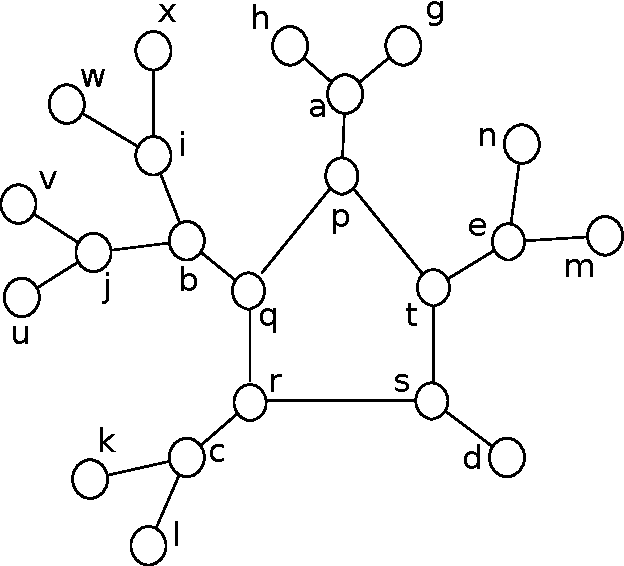
\includegraphics[scale=0.4]{pent} 
%\caption{Pentagon $pqrst$}
%\label{fig:pent}
%\end{center}
%\end{figure}

%\lipsum[1]

%\section{SECTION NAME}
%\lipsum[2]

%\begin{table}
%\centering
%\begin{tabular}{| c | c |}
%\hline
%{\bf item 1} & {\bf item 2} \\ \hline
%
%abcde & 5 \\ \hline
%
%pqrst & 4 \\ \hline
%\end{tabular}
%\caption{A sample table}
%\label{table:1}
%\end{table}
